\documentclass[10pt,DIV16,a4paper,abstract=true,twoside=semi,openright]
{scrreprt}
\usepackage[english]{babel}
\usepackage[numbers, sort&compress]{natbib}
\usepackage{isabelle,isabellesym}
\usepackage{booktabs}
\usepackage{paralist}
\usepackage{graphicx}
\usepackage{amssymb}
\usepackage{xspace}
\usepackage{xcolor}
\usepackage{hyperref}

\sloppy
\pagestyle{headings}
\isabellestyle{default}
\setcounter{tocdepth}{1}
\newcommand{\ie}{i.\,e.\xspace}
\newcommand{\eg}{e.\,g.\xspace}
\newcommand{\thy}{\isabellecontext}
\renewcommand{\isamarkupsection}[1]{%
  \begingroup% 
  \def\isacharunderscore{\textunderscore}%
  \section{#1 (\thy)}%
  \endgroup% 
}

\title{Stateful Protocol Composition and Typing}
\author{%
   \href{https://www.dtu.dk/english/service/phonebook/person?id=64207}{Andreas~V.~Hess}\footnotemark[1]
   \and
   \href{https://people.compute.dtu.dk/samo/}{Sebastian~M{\"o}dersheim}\footnotemark[1]
   \and
   \href{http://www.brucker.ch/}{Achim~D.~Brucker}\footnotemark[2]
}
\publishers{%
  \footnotemark[1]~DTU Compute, Technical University of Denmark, Lyngby, Denmark\texorpdfstring{\\}{, }
   \texttt{\{avhe, samo\}@dtu.dk}\\[2em]
  %
  \footnotemark[2]~
  Department of Computer Science, University of Exeter, Exeter, UK\texorpdfstring{\\}{, }
  \texttt{a.brucker@exeter.ac.uk}
  %
}

\begin{document}
  \maketitle
  \begin{abstract}
    \begin{quote}
        We provide in this AFP entry several relative soundness results for security protocols.
        In particular, we prove typing and compositionality results for stateful protocols (i.e., protocols with mutable state that may span several sessions), and that focuses on reachability properties.
        Such results are useful to simplify protocol verification by reducing it to a simpler problem: Typing results give conditions under which it is safe to verify a protocol in a typed model where only ``well-typed'' attacks can occur whereas compositionality results allow us to verify a composed protocol by only verifying the component protocols in isolation.
        The conditions on the protocols under which the results hold are furthermore syntactic in nature allowing for full automation.
        The foundation presented here is used in another entry to provide fully automated and formalized security proofs of stateful protocols.

    \bigskip
    \noindent{\textbf{Keywords:}} 
    Security protocols, stateful protocols, relative soundness results, proof assistants, Isabelle/HOL, compositionality
    \end{quote}
  \end{abstract}


\tableofcontents
\cleardoublepage

\chapter{Introduction}
The rest of this document is automatically generated from the formalization in Isabelle/HOL, i.e., all content is checked by Isabelle.
The formalization presented in this entry is described in more detail in several publications:
\begin{itemize}
\item The typing result (\autoref{sec:Typing-Result} ``Typing\_Result'') for stateless protocols, the TLS formalization (\autoref{sec:Example-TLS} ``Example\_TLS''), and the theories depending on those (see \autoref{fig:session-graph}) are described in~\cite{hess.ea:formalizing:2017} and~\cite[chapter 3]{hess:typing:2018}.
\item The typing result for stateful protocols (\autoref{sec:Stateful-Typing} ``Stateful\_Typing'') and the keyserver example (\autoref{sec:Example-Keyserver} ``Example\_Keyserver'') are described in~\cite{hess.ea:typing:2018} and~\cite[chapter 4]{hess:typing:2018}.
\item The results on parallel composition for stateless protocols (\autoref{sec:Parallel-Compositionality} ``Parallel\_Compositionality'') and stateful protocols (\autoref{sec:Stateful-Compositionality} ``Stateful\_Compositionality'') are described in~\cite{hess.ea:stateful:2018} and~\cite[chapter 5]{hess:typing:2018}.
\end{itemize}
Overall, the structure of this document follows the theory dependencies (see \autoref{fig:session-graph}): we start with introducing the technical preliminaries of our formalization (\autoref{cha:preliminaries}).
Next, we introduce the typing results in \autoref{cha:typing} and \autoref{cha:stateful-typing}.
We introduce our compositionality results in \autoref{cha:composition} and \autoref{cha:stateful-composition}.
Finally, we present two example protocols \autoref{cha:examples}.

\paragraph{Acknowledgments}
This work was supported by the Sapere-Aude project ``Composec: Secure Composition of Distributed Systems'', grant 4184-00334B of the Danish Council for Independent Research.

\clearpage

\begin{figure}
  \centering
  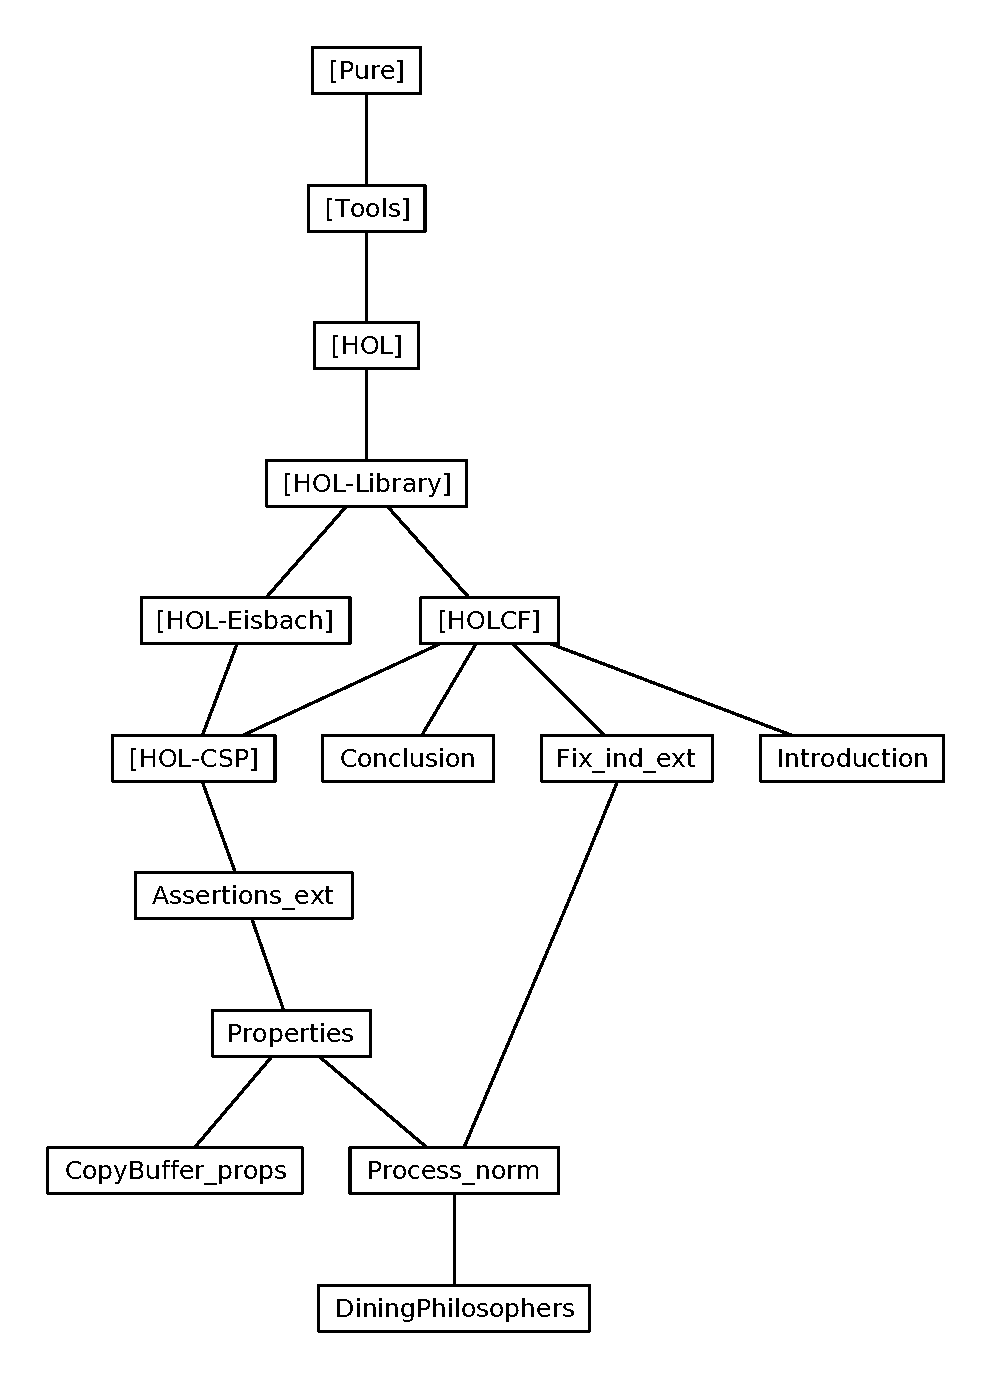
\includegraphics[height=\textheight]{session_graph}
  \caption{The Dependency Graph of the Isabelle Theories.\label{fig:session-graph}}
\end{figure}

\clearpage

% \input{session}

\chapter{Preliminaries and Intruder Model}
\label{cha:preliminaries}
In this chapter, we introduce the formal preliminaries, including the intruder model and related lemmata.
\input{Miscellaneous.tex}
\input{Messages.tex}
\input{More_Unification.tex}
\input{Intruder_Deduction.tex}

\chapter{The Typing Result for Non-Stateful Protocols}
\label{cha:typing}
In this chapter, we formalize and prove a typing result for ``stateless'' security protocols.
This work is described in more detail in~\cite{hess.ea:formalizing:2017} and~\cite[chapter 3]{hess:typing:2018}.
\input{Strands_and_Constraints.tex}
\input{Lazy_Intruder.tex}
\input{Typed_Model.tex}
\input{Typing_Result.tex}

\chapter{The Typing Result for Stateful Protocols}
\label{cha:stateful-typing}
In this chapter, we lift the typing result to stateful protocols.
For more details, we refer the reader to~\cite{hess.ea:typing:2018} and~\cite[chapter 4]{hess:typing:2018}.
\input{Stateful_Strands.tex}
\input{Stateful_Typing.tex}

\chapter{The Parallel Composition Result for Non-Stateful Protocols}
\label{cha:composition}
In this chapter, we formalize and prove a compositionality result for security protocols.
This work is an extension of the work described in~\cite{hess.ea:stateful:2018} and~\cite[chapter 5]{hess:typing:2018}.
\input{Labeled_Strands.tex}
\input{Parallel_Compositionality.tex}

\chapter{The Stateful Protocol Composition Result}
\label{cha:stateful-composition}
In this chapter, we extend the compositionality result to stateful security protocols.
This work is an extension of the work described in~\cite{hess.ea:stateful:2018} and~\cite[chapter 5]{hess:typing:2018}.
\input{Labeled_Stateful_Strands.tex}
\input{Stateful_Compositionality.tex}

\chapter{Examples}
\label{cha:examples}
In this chapter, we present two examples illustrating our results:
In \autoref{sec:Example-TLS} we show that the TLS example from~\cite{hess.ea:formalizing:2017} is type-flaw resistant.
In \autoref{sec:Example-Keyserver} we show that the keyserver examples from~\cite{hess.ea:typing:2018,hess.ea:stateful:2018} are also type-flaw resistant and that the steps of the composed keyserver protocol from~\cite{hess.ea:stateful:2018} satisfy our conditions for protocol composition. 
\input{Example_TLS.tex}
\input{Example_Keyserver.tex}

{\small
  \bibliographystyle{abbrvnat}
  \bibliography{root}
}
\end{document}

%%% Local Variables:
%%% mode: latex
%%% TeX-master: t
%%% End:
